

\section{Global pies}

\subsection{Including all}
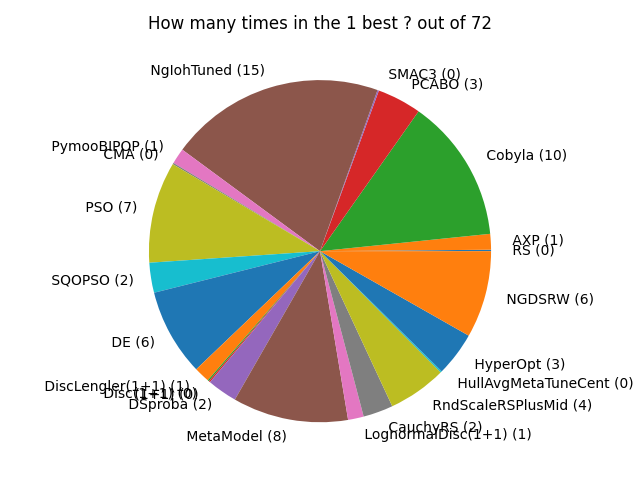
\includegraphics[width=.48\textwidth]{pie1.png}
\includegraphics[width=.48\textwidth]{pie2.png}
\includegraphics[width=.48\textwidth]{pie4.png}
\includegraphics[width=.48\textwidth]{pie8.png}
\subsection{No NgIohTuned, no NGDSRW, only one per category}
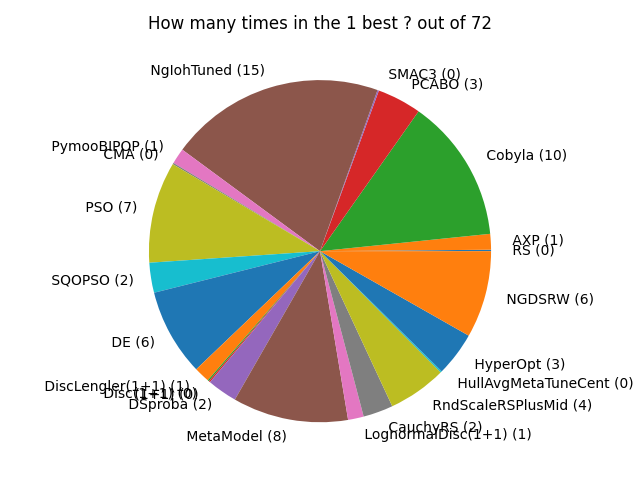
\includegraphics[width=.48\textwidth]{pie1.png}
\includegraphics[width=.48\textwidth]{pie2.png}
\includegraphics[width=.48\textwidth]{pie4.png}
\includegraphics[width=.48\textwidth]{pie8.png}


\section{Comparison with baseline}
\subsection{Comparison for the normalized simple regret}
\input{compa.tex}
\subsection{Comparison for the frequency of outperforming other algorithms}
\input{compa2.tex}

\section*{Acknowledgements}
We are very grateful to the Dagstuhl seminar 23251 (June 2023).%, and more specifically to 

% TODO  done in discussions with with Diederick, Carola
\bibliographystyle{abbrv}
\bibliography{biblio.bib}
\end{document}
